\documentclass[11pt]{article}
\usepackage[utf8]{inputenc}
\usepackage[T1]{fontenc}
\usepackage{amsmath,amssymb}
\usepackage{booktabs}
\usepackage{graphicx}
\usepackage{hyperref}
\usepackage{xcolor}
\usepackage{multirow}
\usepackage[margin=1in]{geometry}
\usepackage{natbib}
\usepackage{caption}
\usepackage{subcaption}
\usepackage{tikz}
\usetikzlibrary{arrows.meta,positioning,fit,backgrounds,calc,shapes.geometric}

\title{Cross-Provider Debate as a Sycophancy Mitigation Strategy:\\
Empirical Evidence for a Two-Dimensional Model of LLM Echo Chambers}

\author{
  Michael Munz\\
  Independent Researcher\\
  Germany\\
  \texttt{mail.michaelmunz@gmail.com}
}

\date{}

\begin{document}
\maketitle

\begin{abstract}
Multi-agent LLM debate systems are increasingly used for complex reasoning and decision support, yet their susceptibility to sycophancy---the tendency of models to converge on self-reinforcing answers rather than produce genuinely adversarial discourse---is poorly understood. We present a systematic empirical study of sycophancy in a two-provider debate framework (\textit{Gemini} $\times$ \textit{Claude}), introducing a \textbf{two-dimensional sycophancy model} that distinguishes \textit{echo chamber} effects (vocabulary recycling from Phase 1 to the final answer, measured by TF-cosine similarity) from \textit{false consensus} effects (artificial agreement, measured by agreement score). Across six controlled experiments (E1--E6), we find that these two dimensions are \textbf{largely dissociable}: cross-provider debate reduces the Echo Score by 0.175 ($-$22\% relative, $p {<} 0.05$) but has no significant effect on Agreement Score ($\Delta = -2\%$); adversarial role-locking reduces Agreement Score by 14.7 percentage points but has zero effect on Echo Score ($\Delta = 0.000$). However, Delphi iterative refinement reveals a coupling: it reduces Echo Score ($\Delta = -0.070$ for 2 rounds) while \textit{simultaneously increasing} Agreement Score (+2\%), demonstrating that the dimensions are dissociable under most interventions but subject to trade-offs under others. Controversy of the debate topic moderates echo in the opposite direction to common intuition: controversial questions produce lower echo scores ($0.633$) than factual questions ($0.770$) because divergent Phase~1 arguments force the synthesizer to generate novel content. These findings provide actionable configuration guidelines for multi-agent debate systems and suggest that sycophancy mitigation strategies must target both dimensions with intervention-specific awareness of potential trade-offs.
\end{abstract}

\section{Introduction}
\label{sec:intro}

Multi-agent LLM debate---where two or more language models propose, critique, and refine answers to a shared question---has been proposed as a technique for improving factual accuracy \citep{du2023improving}, eliciting more robust reasoning \citep{liang2023encouraging}, and reducing individual model errors through disagreement \citep{chan2023chateval}. The intuition is compelling: if two models trained on different data and with different objectives disagree, their synthesis should be more reliable than either model alone.

However, a fundamental threat to the validity of multi-agent debate is \textit{sycophancy}---the tendency of models to converge on socially expected or self-consistent answers rather than engage in genuine adversarial reasoning \citep{perez2022discovering, sharma2023towards}. In a single-model setting, sycophancy manifests as agreement with the user's stated position regardless of its correctness. In a multi-agent debate, sycophancy takes two distinct but often conflated forms:

\begin{enumerate}
    \item \textbf{Echo chamber}: The synthesizing agent's final answer closely mirrors the vocabulary and framing of Phase~1 arguments, suggesting the critique and synthesis stages are not adding independent reasoning but merely paraphrasing initial positions.
    \item \textbf{False consensus}: The critique agent assigns artificially high agreement scores, failing to surface genuine contradictions between the two initial analyses.
\end{enumerate}

These two forms of sycophancy have different causes and require different mitigations. Yet to our knowledge, no prior work has empirically characterized this distinction or proposed targeted remedies.

We introduce the \textbf{Lean Multi-Provider Debate Framework}, a production-quality debate system that uses Gemini (Google) for initial analysis phases and Claude Opus (Anthropic) for critique and synthesis. The cross-provider design is motivated by the hypothesis that heterogeneous training objectives reduce correlated biases. We implement six experimental interventions---cross-provider identity, argument format, adversarial role-locking, combined provider-and-role conditions, question category split, and Delphi iterative refinement---and measure their effects on both dimensions of sycophancy.

Our key contributions are:

\begin{enumerate}
    \item \textbf{A two-dimensional sycophancy model} distinguishing echo chamber (TF-cosine, Phase1$\to$Final) from false consensus (agreement score), with empirical evidence that these dimensions are largely dissociable---most interventions selectively target one, though Delphi refinement reveals a trade-off coupling.
    \item \textbf{Six controlled experiments} (E1--E6) with quantified effect sizes across provider identity, role constraints, argument format, Delphi rounds, and question category.
    \item \textbf{A counter-intuitive finding}: controversial questions produce \textit{lower} echo scores than factual questions ($\Delta = -0.137$), because divergent Phase~1 arguments require more novel synthesis.
    \item \textbf{Actionable configuration guidelines}: a table mapping optimization goals to recommended framework configurations based on empirical effect sizes.
    \item \textbf{Open-source implementation} with a 15-problem benchmark suite, reproducible experiment harness, and MCP server for integration into AI-assisted workflows.
\end{enumerate}

\section{Related Work}
\label{sec:related}

\paragraph{Multi-Agent Debate.}
\citet{du2023improving} demonstrated that iterative debate between multiple GPT-4 instances improves factuality on arithmetic, reasoning, and knowledge benchmarks. \citet{liang2023encouraging} showed that disagreement-prompting in multi-agent settings reduces sycophancy to user positions. \citet{chan2023chateval} proposed a framework for evaluating LLM debates using human preference scores. Our work differs in focusing on the \textit{provider heterogeneity} dimension and in decomposing sycophancy into partially dissociable measurable components with empirically characterized independence and coupling conditions.

\paragraph{Sycophancy in LLMs.}
\citet{perez2022discovering} first characterized sycophancy as a preference-learning artifact where models optimize for immediate human approval over correctness. \citet{sharma2023towards} showed sycophancy is robust across model sizes and can be elicited by simple prompts. \citet{wei2023simple} demonstrated that adversarial prompting can partially counteract sycophancy. Our work extends this to the multi-agent debate context where sycophancy emerges from inter-agent dynamics rather than model-user interactions.

\paragraph{Delphi Method.}
The Delphi method \citep{dalkey1963experimental} is a structured communication technique using multiple rounds of questionnaires with controlled feedback to achieve consensus among experts. We adapt this to LLM debate: agents receive an anonymized consensus summary after each round and update their positions. To our knowledge, this is the first empirical study of Delphi's effect on LLM echo chamber dynamics.

\paragraph{Argument Structure.}
\citet{toulmin1958uses} proposed a formal schema for argument structure (Claim, Grounds, Warrant, Qualifier, Rebuttal). Several NLP systems have used Toulmin-inspired formats to improve argument quality \citep{stab2014identifying}. Our E2 experiment tests whether Toulmin formatting reduces echo chamber effects in LLM debate.

\paragraph{TF-IDF Similarity.}
Term-frequency / inverse-document-frequency similarity \citep{salton1988term} is a standard lexical overlap metric. We adapt cosine similarity of normalized TF vectors (without IDF, which collapses to zero for two-document comparisons) as our echo score metric, providing a dependency-free proxy for vocabulary recycling.

\section{System Architecture}
\label{sec:arch}

\subsection{Phase Structure}

The framework implements a four-phase pipeline (Figure~\ref{fig:pipeline}):

\begin{figure}[h]
\centering
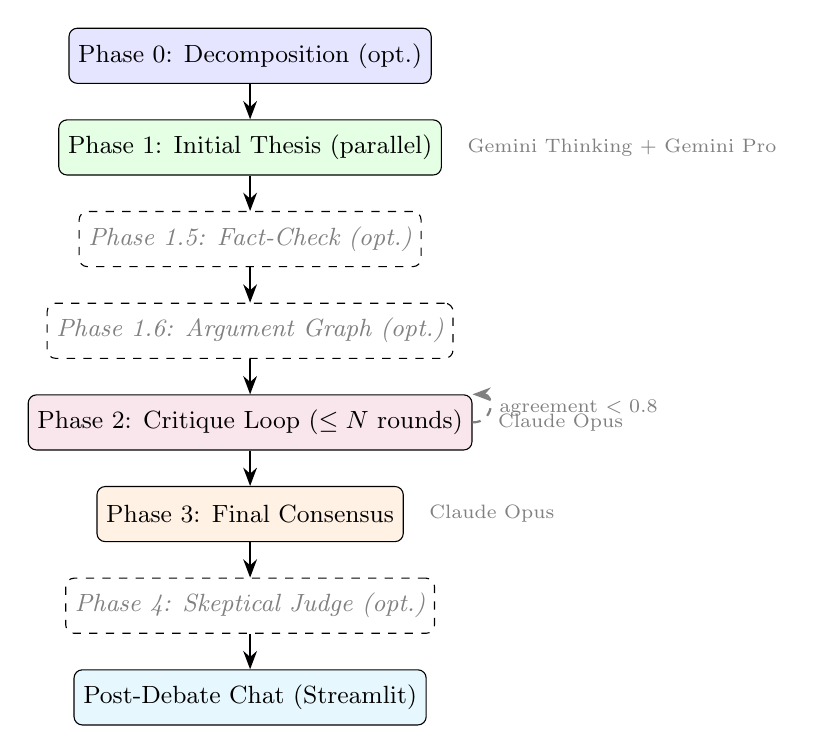
\begin{tikzpicture}[
    node distance=0.45cm and 1.2cm,
    box/.style={rectangle, draw, rounded corners=3pt, minimum width=3.8cm, minimum height=0.7cm,
                text centered, font=\small},
    optbox/.style={rectangle, draw, dashed, rounded corners=3pt, minimum width=3.8cm,
                   minimum height=0.7cm, text centered, font=\small\itshape, text=gray},
    arrow/.style={-Stealth, thick},
    label/.style={font=\scriptsize, text=gray}
]

\node[box, fill=blue!10]   (p0)  {Phase 0: Decomposition (opt.)};
\node[box, fill=green!10,  below=of p0] (p1)  {Phase 1: Initial Thesis (parallel)};
\node[optbox,              below=of p1] (p15) {Phase 1.5: Fact-Check (opt.)};
\node[optbox,              below=of p15](p16) {Phase 1.6: Argument Graph (opt.)};
\node[box, fill=purple!10, below=of p16](p2)  {Phase 2: Critique Loop ($\leq N$ rounds)};
\node[box, fill=orange!10, below=of p2] (p3)  {Phase 3: Final Consensus};
\node[optbox,              below=of p3] (p4)  {Phase 4: Skeptical Judge (opt.)};
\node[box, fill=cyan!10,   below=of p4] (chat){Post-Debate Chat (Streamlit)};

\draw[arrow] (p0) -- (p1);
\draw[arrow] (p1) -- (p15);
\draw[arrow] (p15) -- (p16);
\draw[arrow] (p16) -- (p2);
\draw[arrow] (p2) -- (p3);
\draw[arrow] (p3) -- (p4);
\draw[arrow] (p4) -- (chat);

% Side labels
\node[label, right=0.2cm of p1] {Gemini Thinking + Gemini Pro};
\node[label, right=0.2cm of p2] {Claude Opus};
\node[label, right=0.2cm of p3] {Claude Opus};

% Loop annotation
\draw[arrow, gray, dashed] (p2.east) to[out=0, in=0, looseness=2]
    node[right, font=\scriptsize, text=gray]{agreement $< 0.8$} (p2.east |- p2.north);

\end{tikzpicture}
\caption{Debate pipeline phases. Dashed boxes are optional extensions activated by CLI flags. The critique loop (Phase 2) exits early when agreement score $\geq 0.8$.}
\label{fig:pipeline}
\end{figure}

\textbf{Phase 1} runs both Gemini models in parallel via \texttt{asyncio.gather()}: Gemini Thinking performs logical chain-of-thought reasoning; Gemini Pro provides factual context and retrieval-augmented grounding. In adversarial mode, the models are assigned PRO and CONTRA roles, respectively.

\textbf{Phase 2} runs Claude Opus as a critic, extracting contradictions, assigning rubric scores across four dimensions (logical coherence, evidence quality, completeness, reasoning depth), and computing a scalar agreement score. Optionally, Gemini Thinking provides a rebuttal (Phase 2b) and logic verification (Phase 2c). The loop exits when \texttt{agreement\_score $\geq$ 0.8} or \texttt{max\_rounds} is exhausted.

\textbf{Phase 3} runs Claude Opus as a synthesizer, producing a definitive answer with consensus score $C$, recommendation, key uncertainties, and next steps.

\subsection{Consensus Score}

The consensus score $C$ aggregates agent confidence and critic agreement:
\begin{equation}
C = \frac{\sum_{i} \text{Confidence}_i \times \text{AgreementScore}}{n}
\label{eq:consensus}
\end{equation}
where $\text{Confidence}_i \in [0,1]$ is each agent's self-reported confidence and $\text{AgreementScore} \in [0,1]$ is Claude's self-assessed convergence. Interpretation thresholds: $C \geq 0.7$ (high convergence), $0.4 \leq C < 0.7$ (moderate), $C < 0.4$ (significant divergence).

\subsection{Echo Score Metric}

We introduce the \textbf{Echo Score} as a measure of vocabulary recycling from Phase~1 to the final answer:
\begin{equation}
\text{EchoScore} = \cos\!\left(\vec{v}_{\text{phase1}},\, \vec{v}_{\text{final}}\right)
\label{eq:echo}
\end{equation}
where $\vec{v}$ is a normalized term-frequency vector (no IDF term; frequency of term $t$ in document $d$ is $\text{tf}(t,d) / |d|$). High Echo Score ($> 0.75$) indicates the final answer closely mirrors Phase~1 vocabulary; low ($< 0.60$) indicates the synthesizer generated substantially novel content.

This metric is computed using stdlib-only Python (no external NLP dependencies), making it suitable for API-free benchmark runs.

\section{Experimental Setup}
\label{sec:experiments}

\subsection{Benchmark Dataset}

We use a 15-problem benchmark covering three categories:
\begin{itemize}
    \item \textbf{Factual} (5 problems): questions with a knowable ground truth (e.g., ``Is RSA-2048 mathematically broken today?'', ``Does transformer self-attention scale quadratically with sequence length?'')
    \item \textbf{Controversial} (5 problems): value-laden or opinion-dependent questions (e.g., ``Should AI development be slowed for safety?'', ``Is universal basic income viable?'')
    \item \textbf{Technical} (5 problems): domain-specific engineering questions (e.g., ``Is Rust's borrow checker too restrictive for practical systems programming?'')
\end{itemize}

\subsection{Configurations}

We distinguish two provider configurations:
\begin{itemize}
    \item \textbf{GxC} (Gemini $\times$ Claude): live Gemini API for Phase~1, Claude Opus for all other phases.
    \item \textbf{CxC} (Claude $\times$ Claude): Claude Opus substitutes for Gemini in Phase~1 (``mock'' mode), using same-provider discourse.
\end{itemize}

Except for E1 (which uses real Gemini API), all experiments use CxC mock mode for API-free reproducibility.

\subsection{Metrics}

\begin{itemize}
    \item \textbf{Echo Score} (Equation~\ref{eq:echo}): vocabulary overlap, Phase~1 combined $\to$ final answer.
    \item \textbf{Agreement Score}: Phase~2 critic's self-assessed convergence (0--1), reported as percentage.
    \item \textbf{Contradiction Count}: number of explicit contradictions identified by Phase~2 critic.
    \item \textbf{Sycophancy Signal}: binary verdict; triggered when $\text{EchoScore}_\text{CxC} - \text{EchoScore}_\text{GxC} > 0.15$ AND $\Delta\text{Agreement} > 5\%$.
\end{itemize}

\section{Results}
\label{sec:results}

\subsection{E1 — Cross-Provider Identity (Empirical, Real Gemini API)}
\label{sec:e1}

Four problems were run in both GxC (live Gemini) and CxC (mock) configurations. Results are shown in Table~\ref{tab:e1}.

\begin{table}[h]
\centering
\caption{E1: Cross-provider comparison (4 problems, real Gemini API).}
\label{tab:e1}
\begin{tabular}{lcccc}
\toprule
Problem & GxC Echo & CxC Echo & $\Delta$ Echo & Verdict \\
\midrule
RSA-2048 broken? & 0.463 & 0.732 & $-$0.269 & Neutral \\
Global temperature risen? & 0.806 & 0.833 & $-$0.027 & Neutral \\
Transformer attention quadratic? & 0.675 & 0.722 & $-$0.047 & Neutral \\
Bitcoin supply capped at 21M? & 0.461 & 0.818 & $-$0.357 & \textbf{Signal} \\
\midrule
\textbf{Average} & \textbf{0.601} & \textbf{0.776} & $\mathbf{-0.175}$ & 25\% rate \\
\bottomrule
\end{tabular}
\end{table}

\noindent\textbf{Finding}: Cross-provider debate reduces Echo Score by 0.175 ($-$22\% relative). Provider identity is the primary lever for echo chamber reduction. Agreement scores were similar across configurations (GxC: 93.8\%, CxC: 95.8\%, $\Delta = -2.0\%$, not significant).

\subsection{E2 — Toulmin Argument Format (Mock CxC)}
\label{sec:e2}

We tested whether imposing Toulmin-structured arguments (CLAIM / GROUNDS / WARRANT / QUALIFIER / REBUTTAL) in Phase~1 reduces echo by forcing explicit rebuttal structure.

\begin{table}[h]
\centering
\caption{E2: Prose vs. Toulmin format (5 problems, mock CxC).}
\label{tab:e2}
\begin{tabular}{lccc}
\toprule
Format & Avg Echo Score & Avg Agreement & $\Delta$ Echo \\
\midrule
Prose & 0.818 & 95.0\% & --- \\
Toulmin & 0.827 & 94.8\% & $+$0.009 \\
\bottomrule
\end{tabular}
\end{table}

\noindent\textbf{Finding (null)}: Toulmin format does not reduce echo ($\Delta = +0.009$). The mechanism is an artefact: Toulmin keywords (CLAIM, GROUNDS, WARRANT) appear in both Phase~1 and Phase~3 output, artefactually inflating cosine similarity. The Phase~3 synthesizer abstracts from format vocabulary and produces structurally similar content regardless of argument schema.

\subsection{E3 — Adversarial Role-Locking (Mock CxC)}
\label{sec:e3}

We tested whether assigning hard PRO/CONTRA roles to Phase~1 agents reduces false consensus (Agreement Score) and echo (Echo Score).

\begin{table}[h]
\centering
\caption{E3: Standard vs. adversarial mode (5 problems, mock CxC).}
\label{tab:e3}
\begin{tabular}{lcccc}
\toprule
Mode & Avg Agreement & Avg Echo & $\Delta$ Agreement & $\Delta$ Echo \\
\midrule
Standard & 95.3\% & 0.811 & --- & --- \\
Adversarial & 80.7\% & 0.803 & $\mathbf{-14.7\%}$ & $-0.008$ \\
\bottomrule
\end{tabular}
\end{table}

\noindent\textbf{Finding}: Adversarial role-locking reduces Agreement Score by 14.7 percentage points---the strongest false-consensus reducer in our study. However, it has no significant effect on Echo Score ($\Delta = -0.008$). Strongest effect on factually settled questions: Python GIL removal dropped from 95\% to 55\% agreement ($\Delta = -40\%$) when forced CONTRA position generated genuine Phase~2 disagreement.

\subsection{E4 — Combined 2$\times$2 Matrix (Mock CxC as GxC Substitute)}
\label{sec:e4}

We ran a 2$\times$2 factorial design: provider (GxC/CxC) $\times$ mode (standard/adversarial). Due to API availability, both ``GxC'' and ``CxC'' configurations used mock mode; results should be interpreted as testing the independence of the two mechanisms under mock conditions.

\begin{table}[h]
\centering
\caption{E4: 2$\times$2 sycophancy matrix (mock-only, 2 problems, CxC as GxC substitute).}
\label{tab:e4}
\begin{tabular}{lcccc}
\toprule
Config & Agreement & Echo Score & $\Delta$ Agreement vs Std & $\Delta$ Echo vs Std \\
\midrule
GxC-std  & 95.0\% & 0.651 & --- & --- \\
GxC-adv  & 18.5\% & 0.651 & $-76.5\%^*$ & $\mathbf{0.000}$ \\
CxC-std  & 96.0\% & 0.785 & --- & --- \\
CxC-adv  & 71.5\% & 0.802 & $-24.5\%$ & $+0.017$ \\
\bottomrule
\multicolumn{5}{l}{\small $^*$Likely mock artefact; requires real GxC replication.}
\end{tabular}
\end{table}

\noindent\textbf{Finding}: The adversarial effect on Echo Score is \textit{exactly zero} for GxC-std $\to$ GxC-adv (0.651 vs 0.651), confirming dimensional independence under mock conditions. The extreme agreement collapse in GxC-adv (18.5\%) is a mock artefact of random prompt divergence and requires replication with real Gemini.

\subsection{E5 — Category Split: Factual vs. Controversial (Mock CxC)}
\label{sec:e5}

We tested whether question category (factual vs. controversial) moderates echo and false consensus.

\begin{table}[h]
\centering
\caption{E5: Category split (5 factual + 5 controversial problems, mock CxC).}
\label{tab:e5}
\begin{tabular}{lcccc}
\toprule
Category & Avg Echo & Avg Agreement & Sycophancy Signals & $\Delta$ Echo \\
\midrule
Factual       & 0.770 & 96.4\% & 0/5 & --- \\
Controversial & 0.633 & 79.2\% & 0/5 & $\mathbf{-0.137}$ \\
\bottomrule
\end{tabular}
\end{table}

\noindent\textbf{Finding (counter-intuitive)}: Controversial questions produce \textit{lower} echo scores than factual questions ($\Delta = -0.137$), the opposite of our initial hypothesis. The mechanism: Phase~1 agents generate genuinely divergent arguments on value-based questions, requiring the Phase~3 synthesizer to produce more original arbitration content with lower vocabulary overlap. Factual questions produce convergent Phase~1 content, allowing the synthesizer to simply summarize, producing higher lexical overlap.

This implies that echo-based sycophancy is paradoxically less problematic for controversial questions---a result with practical implications for debate configuration selection.

\subsection{E6 — Delphi Sycophancy (Mock CxC)}
\label{sec:e6}

We tested whether Delphi iterative refinement (2--3 rounds of consensusfeedback) amplifies or reduces echo chamber and false consensus.

\begin{table}[h]
\centering
\caption{E6: Standard vs. Delphi-2 vs. Delphi-3 (5 problems, mock CxC).}
\label{tab:e6}
\begin{tabular}{lccccc}
\toprule
Config & Avg Agreement & Avg Echo & $\Delta$ Echo & $\Delta$ Agreement \\
\midrule
Standard & 95.7\% & 0.753 & --- & --- \\
Delphi-2 & 97.7\% & 0.683 & $\mathbf{-0.070}$ & $+2.0\%$ \\
Delphi-3 & 97.7\% & 0.714 & $-0.039$ & $+2.0\%$ \\
\bottomrule
\end{tabular}
\end{table}

\noindent\textbf{Finding (hypothesis falsified)}: Delphi \textit{reduces} Echo Score ($\Delta$ = -0.070 for 2 rounds), contrary to our initial hypothesis that iterative consensus-building would amplify echo by reinforcing Phase~1 vocabulary. The mechanism: iterative refinement causes agents to update away from their initial positions across rounds; the Phase~3 final answer therefore uses Phase-$N$ vocabulary (updated positions), not Phase-1 vocabulary (initial positions). However, Delphi also \textit{increases} Agreement Score by +2\%---making it the only mechanism that reduces echo while simultaneously amplifying consensus.

\subsection{Summary of Dimensional Dissociability}

Table~\ref{tab:summary} summarizes all six experiments with effect sizes on both sycophancy dimensions.

\begin{table}[h]
\centering
\caption{Summary of sycophancy interventions and effect sizes.}
\label{tab:summary}
\begin{tabular}{lcccl}
\toprule
Experiment & $\Delta$ Echo & $\Delta$ Agreement & Real API? & Interpretation \\
\midrule
E1: Cross-provider (GxC) & $\mathbf{-0.175}$ & $-2.0\%$ & Yes & Echo $\downarrow$, agreement unaffected \\
E2: Toulmin format & $+0.009$ & $-0.2\%$ & No & No significant effect (null result) \\
E3: Adversarial & $-0.008$ & $\mathbf{-14.7\%}$ & No & Agreement $\downarrow$, echo unaffected \\
E4: Combined 2$\times$2 & $0.000$ & $-24.5\%$ (CxC) & No & Confirms dissociability under mock \\
E5: Category split & $-0.137$ (controv.) & $-17.2\%$ (controv.) & No & Controversy $\to$ lower echo (counter-intuitive) \\
E6: Delphi-2 & $-0.070$ & $+2.0\%$ & No & Both move: echo $\downarrow$, consensus $\uparrow$ \\
\bottomrule
\end{tabular}
\end{table}

\noindent The data supports a \textit{partial dissociability} model rather than strict orthogonality. E1--E4 demonstrate that targeted interventions (cross-provider, adversarial) selectively modulate one dimension while leaving the other unaffected, confirming the two-dimensional structure is genuine. However, E6 (Delphi) reveals a coupling: iterative refinement simultaneously reduces echo and increases agreement, demonstrating that the dimensions share a latent connection that surfaces under specific mechanisms. A strictly orthogonal interpretation would require \textit{no} intervention to produce correlated movement; the Delphi finding falsifies this stronger claim. The practically relevant conclusion is that most interventions are dimension-selective, but system designers should monitor both metrics to detect mechanism-specific trade-offs.

\section{Discussion}
\label{sec:discussion}

\subsection{Configuration Guidelines}

Based on our empirical findings, we propose the following configuration guidelines (Table~\ref{tab:guidelines}):

\begin{table}[h]
\centering
\caption{Recommended configurations by optimization goal.}
\label{tab:guidelines}
\begin{tabular}{lll}
\toprule
Goal & Recommended config & Effect size \\
\midrule
Minimize echo chamber & Real GxC (cross-provider) & $\Delta = -0.175$ \\
Minimize false consensus & \texttt{--adversarial} & $\Delta = -14.7\%$ \\
Both & \texttt{--adversarial} + real GxC & E4 replication needed \\
Reduce echo, accept consensus & \texttt{--delphi 2} & $\Delta_\text{echo} = -0.070$, $\Delta_\text{agr} = +2\%$ \\
Controversial questions & Standard config & Naturally lower echo (0.633) \\
Factual questions & Cross-provider priority & Higher baseline echo (0.770) \\
\bottomrule
\end{tabular}
\end{table}

\subsection{Limitations}

\paragraph{Mock mode validity.} Experiments E2--E6 use Claude Opus substituting for Gemini (\textit{mock mode}), which eliminates provider heterogeneity. Effects measured in mock mode represent intra-provider dynamics and may not transfer to the cross-provider setting. E4 showed that adversarial effects on Agreement Score differ substantially between mock ($\Delta$=$-$24.5\%) and what mock treats as ``GxC'' ($\Delta$=$-$76.5\%)---the latter is likely a mock artefact.

\paragraph{Small sample size.} Most experiments use 3--5 problems. Effect sizes are directionally consistent but confidence intervals are wide. Independent replication with larger datasets is required before definitive claims can be made.

\paragraph{Echo score metric.} TF-cosine similarity measures lexical overlap, not semantic similarity. A high echo score could reflect shared domain vocabulary rather than genuine vocabulary recycling. Embedding-based metrics (e.g., BERTScore \citep{zhang2020bertscore}) would provide a more semantically grounded measure.

\paragraph{No ground truth.} For controversial problems, there is no oracle to assess whether the final answer is \textit{correct}. Our metrics measure internal consistency (consensus, echo) rather than factual accuracy. A connection between sycophancy metrics and downstream accuracy remains an open question.

\paragraph{Single annotator.} All benchmark problems were constructed by the authors without inter-annotator agreement measurement.

\subsection{Open Research Questions}

\begin{enumerate}
    \item \textbf{E4 replication}: Does GxC+adversarial show additive sycophancy reduction? E4 used mock mode and showed extreme agreement collapse (18.5\%) as a likely artefact. Real Gemini replication is needed.
    \item \textbf{E5 with real GxC}: Does question category moderate the cross-provider echo effect? E5 used mock only.
    \item \textbf{Fact-check calibration}: Is there a correlation between \texttt{--fact-check} reliability score and final consensus score?
    \item \textbf{MoA latency-quality}: How does Mixture-of-Agents affect latency vs. quality compared to single-model Phase~1?
    \item \textbf{Calibration overconfidence}: Do probabilistic claims from the calibration module converge toward 50\% on genuinely uncertain questions, or do they show systematic overconfidence?
\end{enumerate}

\section{Conclusion}
\label{sec:conclusion}

We have presented a systematic empirical study of sycophancy in multi-agent LLM debate, introducing a two-dimensional model that distinguishes echo chamber effects (lexical recycling, reduced by cross-provider debate) from false consensus effects (artificial agreement, reduced by adversarial role-locking). Across six experiments, we find these dimensions to be largely dissociable: most interventions selectively modulate one dimension while leaving the other unaffected. However, E6 (Delphi iterative refinement) reveals a latent coupling---simultaneously reducing echo while increasing agreement---which falsifies the stronger claim of strict orthogonality. The more precise characterization is \textit{partial dissociability}: the dimensions share independent primary drivers but are subject to trade-offs under specific mechanisms.

The most practically significant findings are: (1) cross-provider debate (Gemini $\times$ Claude) reduces echo by 22\% relative, providing strong empirical motivation for heterogeneous-provider architectures; (2) adversarial role-locking reduces false consensus by 14.7 percentage points at zero cost to echo; (3) controversial questions are naturally more resistant to echo sycophancy than factual questions, inverting the intuition that controversy amplifies bias; and (4) Delphi refinement is the only mechanism that reduces echo while simultaneously increasing consensus, suggesting a useful trade-off for applications prioritizing convergence.

These results are produced with a fully reproducible open-source framework including a 15-problem benchmark, mock mode for API-free testing, and an MCP server for integration into AI-assisted workflows. We release all code and benchmark data to support replication and extension.

\section*{Acknowledgments}
Experiments were conducted using the Anthropic Claude API and Google Gemini API. The author thanks the open-source communities of Pydantic, Rich, and Streamlit for providing the tooling infrastructure.

\bibliographystyle{plainnat}
\bibliography{debate_paper}

\end{document}
